\chapter{Experimentos}
\label{cap:capitulo5}

\begin{flushright}
\begin{minipage}[]{10cm}
\emph{No dejes que la teoría te detenga. Actúa y observa qué sucede.}\\
\end{minipage}\\

Richard Branson\\
\end{flushright}

\vspace{1cm}

%Escribe aquí un párrafo explicando brevemente lo que vas a contar en este capítulo. En este capítulo (y quizás alguno más) es donde, por fin, describes detalladamente qué has hecho y qué experimentos has llevado a cabo para validar tus desarrollos.
En este capítulo se tratarán los diferentes experimentos realizados para llevar
a cabo este proyecto, desde las pruebas más básicas, hasta las más elaboradas,
cuyo éxito da lugar al \textit{software} desarrollado y a los resultados
finales.
Así como en las páginas o apartados de la Wiki\footnote{
\href{https://github.com/RoboticsURJC/tfg-unai/wiki}{https://github.com/RoboticsURJC/tfg-unai/wiki}},
este proyecto se ha apoyado en plataformas de documentos gráficos, como YouTube,
en las que se han ido actualizando vídeos de las pruebas explicadas a
continuación, reunidos en una lista de reproducción\footnote{
\href{https://www.youtube.com/watch?v=x8VAZFSAH1w\&list=PL3OZgGkAPYdkHaZFa2naBTB4b5aglx1h4}{https://www.youtube.com/watch?v=x8VAZFSAH1w\&list=PL3OZgGkAPYdkHaZFa2naBTB4b5aglx1h4}}.



\section{Bases y desarrollo del proyecto}
\label{sec:bases}
%Sección sobre swarm_obj_finder

Una de las partes del periodo de prácticas de empresa consistió en probar la
arquitectura \textit{software} del proyecto que ha sido explicada en la Sección
\ref{sec:topologia_sw}, es por ello que se parte de una base sólida y robusta
por la que empezar a hacer pruebas y mejoras.
Este proyecto base se aloja en un repositorio de GitHub\footnote{
\href{https://github.com/USanz/swarm\_obj\_finder}{https://github.com/USanz/swarm\_obj\_finder}}.
El presente trabajo es una continuación de dicho trabajo.
\\

\subsection{Aplicación Swarm Object Finder}
\label{sec:swarm_obj_finder}

Esta aplicación consiste en la búsqueda y acercamiento a un objeto por múltiples
robots, para demostrar la posibilidad del uso y programación de flujos de datos
con Zenoh-Flow y ROS2 en conjunto.
\\

El funcionamiento interno puede verse resumido en la Figura
\ref{fig:data_flow_scheme}, en la que se aprecian las distintas conexiones entre
los nodos de Zenoh-Flow.
Los robots comienzan dividiéndose el mapa (nodo \textit{Paths Planner}) para
recorrerlo punto por punto de manera controlada y sincronizada (nodo
\textit{Navigator}).
Durante este proceso, se obtiene la información intrínseca de las cámaras, así
como sus imágenes, con las que se detecta el objeto en cuestión (nodo
\textit{Object Detector}) y se infiere su posición (nodo \textit{Object Position
Infering}), para ser enviada al nodo \textit{Navigator}, que se encarga de hacer
que los robots dejen de seguir sus rutas predeterminadas para comenzar a
acercarse al objeto.
Todo ello queda explicado en profundidad en la Wiki\footnote{
\href{https://github.com/RoboticsURJC/tfg-unai/wiki/10.-Migraci\%C3\%B3n-de-swarm\_obj\_finder-a-la-nueva-version-de-Zenoh\%E2\%80\%90flow-\%5B20-Ago-\%E2\%80\%90-30-Sep\%5D\#c\%C3\%B3mo-funciona-swarm\_obj\_finder-y-zenoh-flow}{https://github.com/RoboticsURJC/tfg-unai/wiki/10.-Migracion/funcionamiento}}.

\begin{figure} [h!]
  \begin{center}
    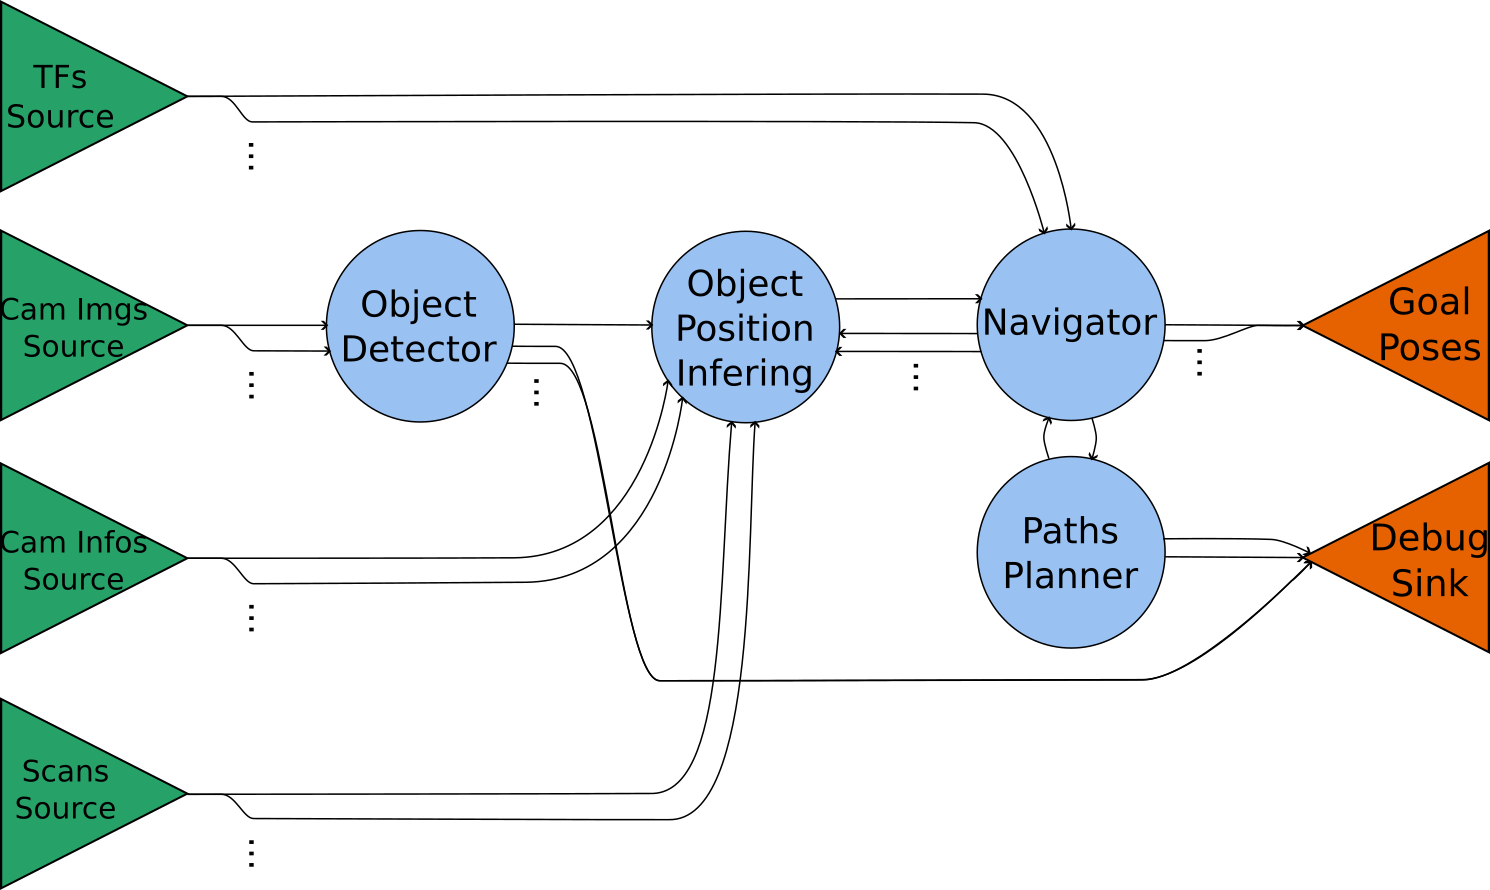
\includegraphics[width=12cm]{figs/data_flow_scheme}
  \end{center}
  \caption{Flujo de datos de la primera versión de \textit{swarm\_obj\_finder}.}
  \label{fig:data_flow_scheme}
\end{figure}\


\subsection{Actualización de Swarm Object Finder}
\label{sec:actualizacion_swarm_obj_finder}

Aunque el funcionamiento de esta arquitectura en simulación fue verificado
durante el periodo de prácticas de empresa, el \textit{software} en conjunto no
funcionaba correctamente al completo, siendo el punto de fallo el \textit{stack}
de navegación, que momentáneamente fallaba a la hora de mover uno de los robots.
Para solucionar este problema se realizaron distintas pruebas, llegando a
contactar con los desarrolladores del \textit{stack} mediante la apertura de un
\textit{Issue} en su repositorio de GitHub\footnote{
\href{https://github.com/ros-navigation/navigation2/issues/3521}{https://github.com/ros-navigation/navigation2/issues/3521}}.
\\

Al no obtener resultados de esta manera se siguió probando hasta que finalmente
se llegó a la solución, actualizando Nav2, el \textit{stack} de navegación, de
su rama ``Foxy'' a ``Humble'', y consecuentemente actualizando ROS a esta misma
distribución, lo que a su vez implicaba actualizar el sistema operativo Ubuntu
de la versión 20.04 a la 22.04.
\\

Además, se actualizó la versión de Zenoh-Flow utilizada en el repositorio
original a una posterior (0.7.2-rc), en la que se solucionaban varios errores y
\textit{bugs}, además de mejorar varios apartados de la API en relación con las
entradas y salidas, así como en la definición del flujo de datos, que queda
explicado más profundamente en la Wiki\footnote{
\href{https://github.com/RoboticsURJC/tfg-unai/wiki/10.-Migraci\%C3\%B3n-de-swarm\_obj\_finder-a-la-nueva-version-de-Zenoh\%E2\%80\%90flow-\%5B20-Ago-\%E2\%80\%90-30-Sep\%5D\#actualizaci\%C3\%B3n-de-swarm\_obj\_finder-a-la-nueva-versi\%C3\%B3n-de-zenoh-flow}{https://github.com/RoboticsURJC/tfg-unai/wiki/10.-Migracion/actualizacion-swarm\_obj\_finder}}.
Consecuentemente, se actualizaron la versión de Zenoh y del \textit{bridge} de
Zenoh, así como de la API de Python, a versiones compatibles con esta nueva
versión de Zenoh-Flow.
\\

\subsection{Mejoras de Swarm Object Finder}
\label{sec:mejoras_swarm_obj_finder}

Una vez se tuvo la aplicación funcionando de nuevo con versiones posteriores de
las herramientas \textit{software} utilizadas, se procedió a su optimización,
eliminando posibles puntos de fallo y enriqueciendo su funcionalidad, aportando
de esta manera mejoras a sus nodos, lo cual también queda detallado en la
Wiki\footnote{
\href{https://github.com/RoboticsURJC/tfg-unai/wiki/11.-Mejoras-y-correcciones-del-swarm\_obj\_finder-\%5B30-Sep-\%E2\%80\%90-9-Nov\%5D}{https://github.com/RoboticsURJC/tfg-unai/wiki/11.-Mejoras-y-correcciones-swarm\_obj\_finder}}.
\\

La primera mejora aplicada va en relación con la creación de distintas clases
con varios objetos, para modularizar el código y mejorar así las comunicaciones
entre los nodos, facilitando la serialización de sus mensajes, lo que da lugar
al módulo \texttt{message\_utils.py}, que se puede observar en el Código
\ref{cod:message_utils}.
En este fragmento observamos la clase \verb|WorldPosition|, que se utiliza
entre los nodos \verb|Navigator| y \verb|PathsPlanner| para informarse de
las posiciones objetivo de los robots en el mundo o para que el nodo
\verb|ObjPosInfer| envié la posición en el mundo del objeto detectado al nodo
\verb|Navigator|.
Así como esta clase, se crearon otras, como la llamada \verb|CentroidMessage|,
para que el nodo \verb|ObjDetector| envíe la posición del objeto detectado al
nodo \verb|ObjPosInfer|.
\\

\begin{code}[h!]
  \begin{lstlisting}[language=Python]
    ...
    class WorldPosition:
        def __init__(self, world_pos:PoseStamped=PoseStamped(), name:str="") -> None:
            self.world_position = world_pos
            self.sender = name
        def set_world_position(self, world_pos:PoseStamped=PoseStamped()) -> None:
            self.world_position = world_pos
        def get_world_position(self) -> PoseStamped:
            return self.world_position
        def set_sender(self, name:str="") -> None:
            self.sender = name
        def get_sender(self) -> str:
            return self.sender
    ...
  \end{lstlisting}
\caption[Clase del objeto \texttt{WorldPosition} del módulo \texttt{message\_utils.py}]{Clase del objeto \texttt{WorldPosition} del módulo \texttt{message\_utils.py}}
\label{cod:message_utils}
\end{code}

Consecuentemente, se desarrolló otro módulo encargado de la serialización de
estos y otros objetos para poder ser enviados entre los nodos, y que además
alberga las funciones de serialización de mensajes de ROS mencionadas en la
Sección \ref{sec:zf_ros}.
Este módulo se llama \texttt{comms\_utils.py} y, como puede verse en el Código
\ref{cod:comms_utils}, serializa los mensajes en función de la longitud del
\texttt{string} del nombre del emisor (``robot1'', ``robot2'', etc.), variable
que será un parámetro fijado en el flujo de datos, determinando esta longitud
máxima para todos los nombres.
\\

\begin{code}[h!]
  \begin{lstlisting}[language=Python]
    ...
    def get_world_pos_msg_serializer(str_bytes_length: int): # Returns a function
        return lambda obj: ser_world_pos_msg(obj, str_bytes_length)
    def ser_world_pos_msg(world_pos_msg: WorldPosition,
                          str_bytes_length: int) -> bytes:
        ser_sender = ser_string(world_pos_msg.sender, str_bytes_length)
        ser_world_pos = ser_ros2_msg(world_pos_msg.world_position)
        return ser_sender + ser_world_pos

    def get_world_pos_msg_deserializer(str_bytes_length: int): # Returns a function
        return lambda obj: deser_world_pos_msg(obj, str_bytes_length)
    def deser_world_pos_msg(world_pos_msg: bytes,
                            str_bytes_length: int) -> WorldPosition:
        ser_sender = world_pos_msg[:str_bytes_length]
        sender = deser_string(ser_sender)
        ser_world_pos = world_pos_msg[str_bytes_length:]
        world_pos = get_ros2_deserializer(PoseStamped)(ser_world_pos)
        return WorldPosition(world_pos, sender)
    ...
  \end{lstlisting}
\caption[Funciones serializadoras del módulo \texttt{comms\_utils.py}]{Funciones serializadoras del módulo \texttt{comms\_utils.py}}
\label{cod:comms_utils}
\end{code}

Además de estos, otros módulos fueron creados, como el módulo
\texttt{map\_utils.py}, el cual ayuda a simplificar y mejorar la conversión
entre los distintos ejes de coordenadas, como los del mapa y los del mundo,
cuyas fórmulas pueden verse en la Ecuación \ref{ec:img_world}.
\\

\begin{myequation}[h!]
  \begin{equation}
  \begin{aligned}
  x_w &= x_i * r + o_x  \\
  y_w &= (h_i - y_i) * r + o_y  \\
  \end{aligned}
  \label{ec:img_world}
  \end{equation}
  \caption[Cambio de ejes de coordenadas de la imagen \textit{i} al mundo \textit{w}]{Cambio de ejes de coordenadas de la imagen \textit{i} al mundo \textit{w}}
\end{myequation}

Este módulo, en el nodo \textit{Paths Planner}, alberga funciones relacionadas
con la división del mapa para la obtención de las rutas formadas por puntos
objetivo en el mundo para cada robot.
Algunas de estas funciones se muestran en el Código \ref{cod:map_utils}.
\\

\begin{code}[h!]
  \begin{lstlisting}[language=Python]
    ...
    def get_squarest_distribution(factors: list) -> list:
        distribution = [1, 1]
        for f in reversed(factors): # Starts from the highest to the lowest.
            if distribution[0] < distribution[1]:
                # The factor is multiplied by the lowest member of the distribution:
                distribution[0] *= f
            else:
                distribution[1] *= f
        return distribution
    ...
    def img2world(img_pix: tuple, img_shape: tuple,
              res: float, origin: tuple) -> tuple:
        # Image needed info:
        xi, yi = img_pix
        hi, _  = img_shape
        # World needed info:
        ox, oy, _ = origin
        # Image pixel to world position conversion:
        xw =       xi  * res + ox
        yw = (hi - yi) * res + oy # Y axis needs to be inverted.
        return (xw, yw)
    ...
  \end{lstlisting}
\caption[Funciones del módulo \texttt{map\_utils.py}]{Funciones del módulo \texttt{map\_utils.py}}
\label{cod:map_utils}
\end{code}

El módulo \texttt{geom\_utils.py} se encarga de funciones matemáticas
relacionadas con la geometría, albergando todos los cálculos relacionados con
cuaterniones, como las que pueden verse en la Ecuación \ref{ec:quat_to_euler}.
En esta ecuación de ejemplo se está infiriendo la posición del objeto en el nodo
\verb|ObjPosInfer|, lo cual se muestra en el código \ref{cod:geom_utils}.
Asimismo, su operación inversa se representa en la Ecuación
\ref{ec:euler_to_quat}.
\\

\begin{myequation}[h!]
  \begin{equation}
  \begin{aligned}
  q_x &= \sin{\frac{r}{2}} * \cos{\frac{p}{2}} * \cos{\frac{y}{2}} - \cos{\frac{r}{2}} * \sin{\frac{p}{2}} * \sin{\frac{y}{2}}  \\
  q_y &= \cos{\frac{r}{2}} * \sin{\frac{p}{2}} * \cos{\frac{y}{2}} + \sin{\frac{r}{2}} * \cos{\frac{p}{2}} * \sin{\frac{y}{2}}  \\
  q_z &= \cos{\frac{r}{2}} * \cos{\frac{p}{2}} * \sin{\frac{y}{2}} - \sin{\frac{r}{2}} * \sin{\frac{p}{2}} * \cos{\frac{y}{2}}  \\
  q_w &= \sin{\frac{r}{2}} * \cos{\frac{p}{2}} * \cos{\frac{y}{2}} + \sin{\frac{r}{2}} * \sin{\frac{p}{2}} * \sin{\frac{y}{2}}  \\
  \end{aligned}
  \label{ec:quat_to_euler}
  \end{equation}
  \caption[Obtención de cuaterniones a partir de ángulos de Euler (RPY)]{Obtención de cuaterniones a partir de ángulos de Euler (RPY)}
\end{myequation}

\begin{code}[h!]
  \begin{lstlisting}[language=Python]
    ...
    def euler2quat(rpy: tuple) -> Quaternion:
        roll, pitch, yaw = rpy
        qx = math.sin(roll/2) * math.cos(pitch/2) * math.cos(yaw/2) - math.cos(roll/2) * math.sin(pitch/2) * math.sin(yaw/2)
        qy = math.cos(roll/2) * math.sin(pitch/2) * math.cos(yaw/2) + math.sin(roll/2) * math.cos(pitch/2) * math.sin(yaw/2)
        qz = math.cos(roll/2) * math.cos(pitch/2) * math.sin(yaw/2) - math.sin(roll/2) * math.sin(pitch/2) * math.cos(yaw/2)
        qw = math.cos(roll/2) * math.cos(pitch/2) * math.cos(yaw/2) + math.sin(roll/2) * math.sin(pitch/2) * math.sin(yaw/2)
        return Quaternion(x=qx, y=qy, z=qz, w=qw)

    def quat2euler(q: Quaternion) -> tuple:
        x = math.atan2(2 * (q.w*q.x + q.y*q.z), (1 - 2 * (q.x**2 + q.y**2)))
        y = -math.pi/2 + 2* math.atan2(math.sqrt(1+2*(q.w*q.y-q.x*q.z)), math.sqrt(1-2*(q.w*q.y-q.x*q.z)))
        z = math.atan2(2*(q.w*q.z + q.x*q.y), 1-2*(q.y**2 + q.z**2))
        return (x, y, z)
    ...
  \end{lstlisting}
\caption[Funciones matemáticas del módulo \texttt{geom\_utils.py}]{Funciones matemáticas del módulo \texttt{geom\_utils.py}}
\label{cod:geom_utils}
\end{code}

\begin{myequation}[h!]
  \begin{equation}
  \begin{aligned}
  x &= \tan{\frac{2 * (q_w*q_x + q_y*q_z)}{1 - 2 * (q_x^2 + q_y^2)}}  \\
  y &= -\frac{\pi}{2} * \tan{\sqrt{1 + 2 * (q_w * q_y - q_x * q_z)}}{\sqrt{1 - 2 * (q_w * q_y - q_x * q_z)}}  \\
  z &= \tan{\frac{2 * (q_w * q_z + q_x * q_y)}{1 - 2 * (q_y^2 + q_z^2)}}  \\
  \end{aligned}
  \label{ec:euler_to_quat}
  \end{equation}
  \caption[Obtención de ángulos de Euler (RPY) a partir de Cuaterniones]{Obtención de ángulos de Euler (RPY) a partir de Cuaterniones}
\end{myequation}



\section{Pruebas en simulación}
\label{sec:pruebas_sim}

Además de los cambios anteriores, también se modificó el modelo del Turtlebot 3
\textit{waffle} simulado, en el repositorio del \textit{stack} de navegación
Nav2, ya que la posición de su sensor LIDAR virtual no era la misma que la de su
modelo 3D y, al estar situado más alto, no permitía la detección mutua entre los
robots.
En la Figura \ref{fig:mutua_deteccion} se aprecia el problema descrito: los
rayos emitidos por el sensor, en la parte izquierda de la figura no corresponden
con el propio sensor, mientras que sí lo hacen correctamente en la parte derecha
de la figura, tras haber modificado su posición.
Este cambio también fue explicado en la Wiki\footnote{
\href{https://github.com/RoboticsURJC/tfg-unai/wiki/8.-Soluci\%C3\%B3n-del-problema-de-mutua-detecci\%C3\%B3n-de-los-Turtlebot3-\%5B28-Jun---29-Jul\%5D}{https://github.com/RoboticsURJC/tfg-unai/wiki/8.-Solucion-problema-deteccion}}.

\begin{figure} [h!]
  \begin{center}
    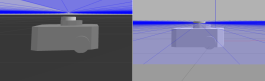
\includegraphics[width=12cm]{figs/turtlebot_model_mods}
  \end{center}
  \caption{Modelos 3D del robot antes (izq.) y después (dcha.) de modificar el sensor.}
  \label{fig:mutua_deteccion}
\end{figure}\

Así como la corrección de varios \textit{bugs} y mejoras de la información
mostrada por la interfaz, también se modificó la forma de obtención de los datos
de profundidad en el momento de detección del objeto, ya que en el repositorio
original eran obtenidos utilizando las medidas del sensor LIDAR, al haber sido
desarrollado en un principio para un robot Turtlebot 3 modelo \textit{burger}
real, el cual no tenía cámara de profundidad.
\\

Puesto que ahora se utilizan robots Turtlebot 3 modelo \textit{waffle}
simulados, que sí incluyen una cámara RGBD, y por tanto son capaces de detectar
profundidad en sus imágenes, ya no se necesitarán las medidas del láser para
este propósito.
El nuevo modelo de obtención de profundidad, únicamente a partir de los datos de
la cámara, se puede observar en la Figura \ref{fig:coords_infer}, mediante la
aplicación de cambios de ejes de coordenadas y trigonometría, y que queda
explicado en la Wiki\footnote{
\href{https://github.com/RoboticsURJC/tfg-unai/wiki/11.-Mejoras-y-correcciones-del-swarm\_obj\_finder-\%5B30-Sep-\%E2\%80\%90-9-Nov\%5D\#cambios-del-nodo-detector-de-objetos}{https://github.com/RoboticsURJC/tfg-unai/wiki/11.-Mejoras/\#cambios-nodo-detector}}.
\\

\begin{figure} [h!]
  \begin{center}
    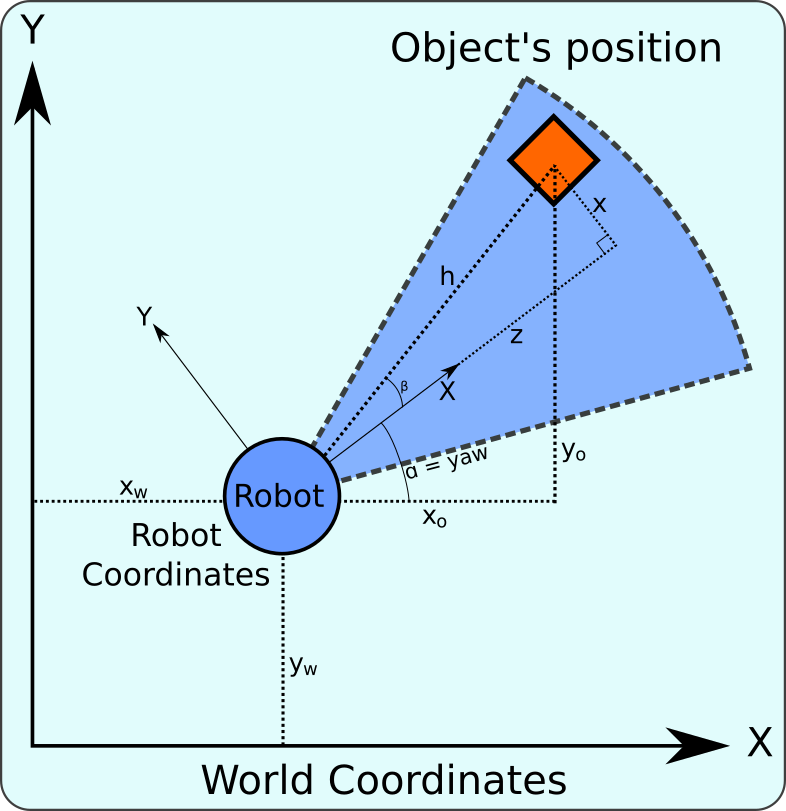
\includegraphics[width=7cm]{figs/coordinates_scheme}
  \end{center}
  \caption{Inferencia de las coordenadas del objeto detectado.}
  \label{fig:coords_infer}
\end{figure}\

En cuanto al módulo de navegación, se realizaron los cambios necesarios para
sustituir el comportamiento caótico de los robots al detectar el objeto, ya que
todos los que lo detectaban ordenaban al resto moverse a una posición cercana al
objeto, a una distancia de seguridad.
Dicho cambio también queda reflejado en la Wiki\footnote{
\href{https://github.com/RoboticsURJC/tfg-unai/wiki/11.-Mejoras-y-correcciones-del-swarm\_obj\_finder-\%5B30-Sep-\%E2\%80\%90-9-Nov\%5D\#cambio-en-la-l\%C3\%B3gica-del-algoritmo-en-el-modo-de-acercamiento-al-objeto}{https://github.com/RoboticsURJC/tfg-unai/wiki/11.-Mejoras/\#cambio-algoritmo-acercamiento}}.
Al ser detectado desde posiciones o puntos de vista distintos, las posiciones
seguras inferidas diferían ligeramente dependiendo de la posición del robot que
lo detectase y, al ser enviadas continuamente, todos los robots recalculaban su
ruta al objeto por cada vez que uno de ellos enviaba su posición.
\\

Este problema se soluciona con la implementación de un sistema jerárquico o de
preferencias, en el que se asigna el rol de máster al primer robot que detecta
el objeto, y este será el único que podrá enviar la posición del objeto desde su
punto de vista.
El rol de máster solo se cambiará, siendo otorgado a otro robot, en caso de que
el robot con dicho rol pierda de vista al objeto el suficiente tiempo como para
considerar que lo ha perdido, siendo este sistema robusto a cambios de posición
del objeto y a oclusiones del mismo durante la ruta.
Las diferencias entre estos dos métodos puede verse representada en la Figura
\ref{fig:navigator_versions} y, así como en la Wiki, también se han actualizado
documentos gráficos en YouTube\footnote{
\href{https://www.youtube.com/watch?v=pQUbj2aZCQs}{https://www.youtube.com/watch?v=pQUbj2aZCQs}},
consiguiéndose así una prueba gráfica de los resultados descritos.
\\

\begin{figure} [h!]
  \begin{center}
    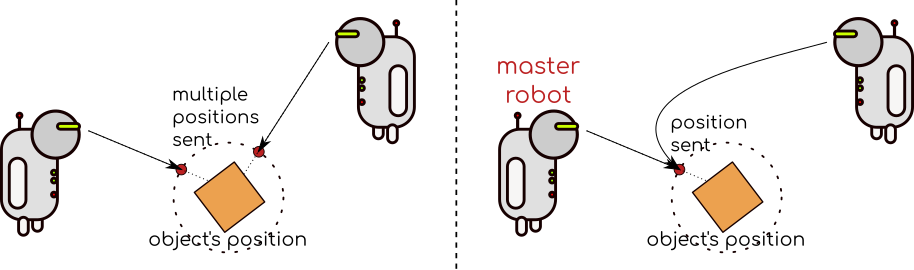
\includegraphics[width=15cm]{figs/navigator_versions}
  \end{center}
  \caption{Representación de las diferentes versiones del nodo \texttt{Navigator}.}
  \label{fig:navigator_versions}
\end{figure}\



\section{Pruebas en un entorno real}
\label{sec:pruebas_real}

En esta sección se explicarán las pruebas y modificaciones realizadas para
trasladar los anteriores resultados conseguidos en simulación a un entorno real
de laboratorio con robots físicos.
\\

\subsection{Pruebas de telecomunicaciones}
\label{sec:pruebas_telecoms}

En primer lugar se debió asegurar que, tanto el entorno \textit{software} como
el entorno \textit{hardware} era apto para el despliegue de la topología
\textit{software} descrita en la Sección \ref{sec:topologia_sw}, con lo que se
llevaron a cabo pruebas de conexión de las distintas máquinas mediante el uso de
\textit{routers} de Zenoh y sus \textit{bridges}, lo cual queda descrito en la
Wiki\footnote{
\href{https://github.com/RoboticsURJC/tfg-unai/wiki/12.-Instalaci\%C3\%B3n-del-software-en-Raspberry-Pi--\%5B9-Nov-\%E2\%80\%90-18-Nov\%5D}{https://github.com/RoboticsURJC/tfg-unai/wiki/12.-Instalacion-software-Raspberry-Pi}}.
\\

Las pruebas mencionadas a nivel de comunicaciones básicas se llevaron a cabo
en distintos pasos, el primero de estos fue probar las comunicaciones básicas
entre el ordenador portátil principal con una Raspberry Pi mediante SSH (Secure
Shell, protocolo que permite acceder remotamente a una máquina), para configurar
el \textit{firewall} del portátil (ya que la Raspberry Pi lo tiene desactivado por
defecto) y que las comunicaciones en ambas direcciones sean posibles.
\\

Una vez accedido a una terminal de la Raspberry Pi desde el ordenador principal,
se pueden lanzar comandos para instalar el software necesario y cambiar su RMW a
CycloneDDS, para lo que se realizaron pruebas únicamente utilizando nodos de
ROS2 mediante los siguientes comandos, uno en cada máquina:
\begin{lstlisting}[language=bash]
  RMW_IMPLEMENTATION=rmw_cyclonedds_cpp ros2 run demo_nodes_py talker
  RMW_IMPLEMENTATION=rmw_cyclonedds_cpp ros2 run demo_nodes_py listener
\end{lstlisting}

Teniendo este ejemplo funcionando correctamente, se hizo la prueba para conectar
estos nodos a través del bridge de Zenoh, lo que se consiguió ejecutando en una
de las máquinas los siguientes comandos:
\begin{lstlisting}[language=bash]
  ./zenoh-bridge-dds -d 1 -l tcp/0.0.0.0:7447
  ROS_DOMAIN_ID=1 ros2 run turtlesim turtlesim_node
\end{lstlisting}

Mientras que en la otra máquina se ejecutan los mismos comandos pero con el nodo
emisor de mensajes:
\begin{lstlisting}[language=bash]
  ./zenoh-bridge-dds -d 2 -e tcp/192.168.1.138:7447
  ROS_DOMAIN_ID=2 ros2 run turtlesim turtle_teleop_key
\end{lstlisting}

El argumento \verb|-d 2|, así como la variable global \verb|ROS_DOMAIN_ID=2|,
permiten correr el nodo y el \textit{bridge} en un dominio distinto al de la
anterior máquina, para asegurarnos que no se conectan mediante DDS, sino que
pasan por el \textit{bridge} para ser traducido y enviado usando Zenoh.
Por supuesto, estas pruebas se realizaron también en sentido contrario,
permitiendo de esta manera la comunicación bidireccional.
\\

Añadiremos ahora Zenoh-Flow a la ecuación, para lo que necesitaremos correr
además del \textit{bridge}, un \textit{router} de Zenoh, lo que se consigue
ejecutando en la Raspberry Pi los siguientes comandos:
\begin{lstlisting}[language=bash]
  zenohd -c ./zenoh_nodes/zenoh_rpi_config.json
  ./zenoh-bridge-dds-0.7.2-rc -e tcp/<ip_portatil>:7447
  ros2 run demo_nodes_py listener
\end{lstlisting}

Siendo la configuración mencionada la mostrada en el Código
\ref{cod:rpi_config}, con la debida sustitución de la etiqueta
\verb|<ip_portatil>| por la IP del portátil en la subred en cuestión.
\\

\begin{code}[h!]
  \begin{lstlisting}[style=json]
    {
        "listen":{
            "endpoints":["tcp/0.0.0.0:7447"]
        },
        "connect":{
            "endpoints":["tcp/<ip_portatil>:7447"]
        }
    }
  \end{lstlisting}
\caption[Configuración del \textit{router} de Zenoh en la Raspberry Pi]{Configuración del \textit{router} de Zenoh en la Raspberry Pi}
\label{cod:rpi_config}
\end{code}


Además, se deberán ejecutar los siguientes comandos en el portátil:
\begin{lstlisting}[language=bash]
  RUST_LOG=zenoh_flow=debug zenohd -c ./zenoh_nodes/zenoh_laptop_config.json
  zf_uuid=$(zfctl launch ./zenoh_nodes/zenoh_flow_tests/data-flow.yaml)
\end{lstlisting}

Siendo esta configuración del portátil la mostrada en el Código
\ref{cod:laptop_config}, sustituyendo las etiquetas \verb|<rpi_ip1>| y
\verb|<rpi_ip2>| por las IPs de las distintas máquinas Raspberry Pi:
\\

\begin{code}[h!]
  \begin{lstlisting}[style=json]
    {
      "listen":{"endpoints":["tcp/0.0.0.0:7447"]},
      "connect":{"endpoints":["tcp/<rpi_ip1>:7447", "tcp/<rpi_ip2>:7447"]},
      "plugins_search_dirs":["/usr/lib/"],
      "plugins":{
          "storage_manager":{
              "required":true,
              "storages":{
                  "zfrpc":{
                      "key_expr":"zf/runtime/**",
                      "volume": "memory"
                      },
                  "zf":{
                      "key_expr":"zenoh-flow/**",
                      "volume": "memory"
                      }
                  }
          },
          "zenoh_flow":{
              "required":true,
              "name":"computer",
              "path":"/etc/zenoh-flow",
              "pid_file": "/var/zenoh-flow/runtime.pid",
              "extensions": "/etc/zenoh-flow/extensions.d",
              "worker_pool_size":4,
              "use_shm": false
          }
      }
  }
  \end{lstlisting}
\caption[Configuración del \textit{router} de Zenoh en la Raspberry Pi]{Configuración del \textit{router} de Zenoh en la Raspberry Pi}
\label{cod:laptop_config}
\end{code}

Con estas pruebas funcionando correctamente, se pueden realizar pruebas en las
que publicar desde Zenoh-Flow una posición objetivo a los nodos de ROS de
navegación de los robots para verlos en movimiento.
Esto puede hacerse creando un data-flow muy sencillo que albergue un nodo
\texttt{operator}, que creará y serializará un mensaje, enviándolo a un nodo
\texttt{sink}, que tendrá como \texttt{key-expression}
``\texttt{rt/robot1/goal\_pose}'', por lo que será entendida y traducida por el
\texttt{bridge} y, por tanto, enviada a los nodos de ROS mencionados mediante
DDS, como ya se ha explicado en las Secciones \ref{sec:zenoh_flow} y
\ref{sec:zf_ros} del capítulo anterior.
\\

Los resultados de esta prueba pueden verse en vídeo\footnote{
\href{https://www.youtube.com/watch?v=upLP5MzOfKo}{https://www.youtube.com/watch?v=upLP5MzOfKo}},
en el que se observa cómo cada robot se dirige a un punto del mapa distinto,
uniendo en esta prueba todas las herramientas \texttt{software} usadas en este
trabajo y demostrando por tanto el funcionamiento de la topología
\texttt{software} explicada en la Sección \ref{sec:topologia_sw}.
\\

La prueba mencionada se llevó a cabo con dos robots distintos (Turtlebot 2 y 4),
ya que al realizar la prueba con dos robots Turtlebot 4, sus ordenadores de a
bordo (Raspberry Pi) no tenían capacidad suficiente para procesar la gran
cantidad de mensajes generados, y por ello dejaban de responder en cuanto se
iniciaban los nodos de navegación de ROS en ambas máquinas y, por tanto, los
nodos receptores de estos mensajes dejaban de recibir información.
\\

Para consolidar esta teoría se realizó una prueba\footnote{
\href{https://www.youtube.com/watch?v=OQEbhof4IFQ}{https://www.youtube.com/watch?v=OQEbhof4IFQ}}
con dichas máquinas, en la que se lanzaron los nodos mencionados y se supervisó
su envío de mensajes con la herramienta \textit{software} PlotJuggler, que
permitió visualizar los mensajes recibidos de los robots, dando lugar a la
gráfica mostrada en la Figura \ref{fig:navigator_versions}.
En concreto, los mensajes de esta gráfica representan la distancia medida con su
sensor láser, que varía debido a la rotación continua del robot, y que comienza
a ralentizarse cuando la navegación de uno de los robots es lanzada, como puede
verse en la gráfica azul, donde se aprecia una menor cantidad de mensajes
recibidos por unidad de tiempo, e incluso dejan de ser recibidos cuando se
activa la navegación del segundo robot, como puede verse en la gráfica roja.
\\

\begin{figure} [h!]
  \begin{center}
    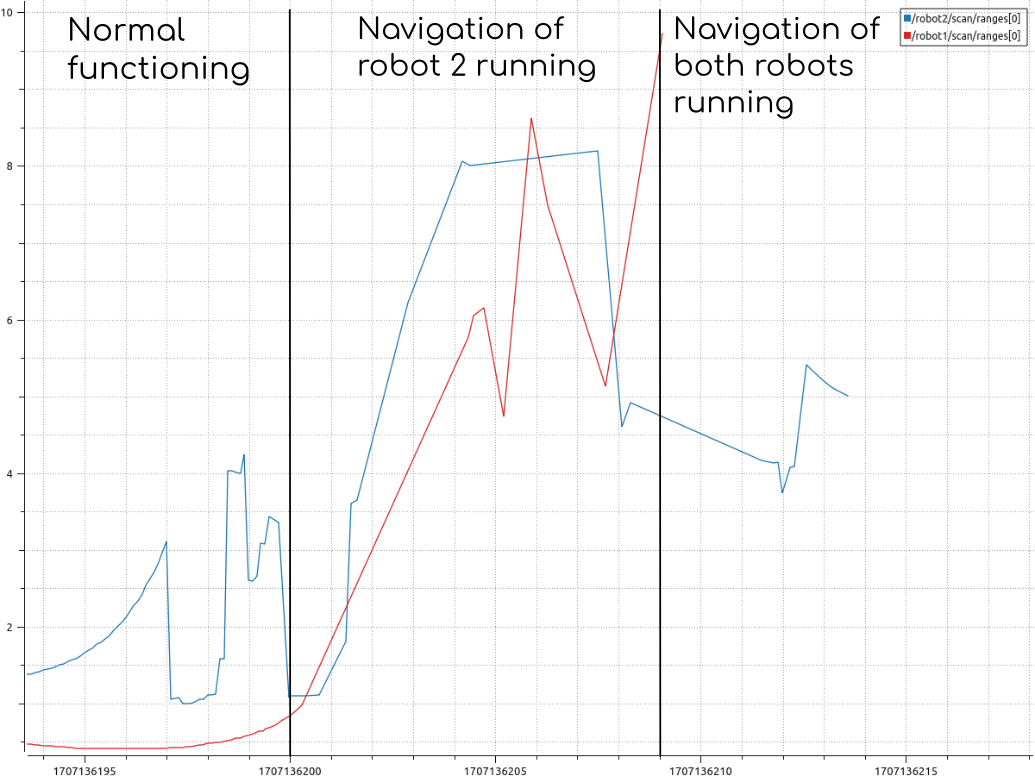
\includegraphics[width=12cm]{figs/plot_congestion_explained}
  \end{center}
  \caption{Comparación de mensajes variando la cantidad de robots.}
  \label{fig:plot_congestion}
\end{figure}\


\subsection{Pruebas de la aplicación}
\label{sec:pruebas_app}

Una vez realizadas las pruebas anteriores se prosiguió con las pruebas de la
aplicación \textit{swarm\_obj\_finder} en los robots reales que, como se ha
explicado en la Sección \ref{sec:bases}, debe dividir la sala y enviar a cada
robot por una ruta de búsqueda en ese área en busca de un objeto.
\\

Primero se llevó a cabo la prueba sin la detección de objetos\footnote{
\href{https://www.youtube.com/watch?v=M8LTSM-3-Es}{https://www.youtube.com/watch?v=M8LTSM-3-Es}},
para evitar posibles errores o saturación de red, por lo que los robots
únicamente debían seguir la ruta proporcionada por el nodo de Zenoh-Flow
\verb|PathsPlanner|.
Dicha prueba, tras algunos cambios menores fue llevada a cabo sin mayor
problema, como también puede verse en el vídeo enlazado.
Esta prueba también demuestra la fácil modularización de Zenoh-Flow, en cuya
estructura podemos cambiar unos nodos por otros sencillamente, o como en este
caso, eliminarlos del flujo de datos.
\\

Para añadir la detección de objetos a nuestra prueba se debieron probar las
distintas cámaras, Orbbec Astra y Asus Xtion, en ambos robots, Turtlebot 2 y 4.
Adicionalmente, se añadió la cámara Oak-D a las pruebas del robot Turtlebot 4,
ya que viene integrada en el mismo.
\\

En cuanto al robot Turtlebot 4, con la cámara Oak-D no se consiguió hacer
funcionar la profundidad; es decir, no se pudo obtener los datos de distancias
de la cámara RGBD, aún habiendo probado distintas configuraciones de la misma
con distintos comandos de los paquetes oficiales \texttt{depthai\_ros\_driver} y
\texttt{turtlebot4\_bringup}, debido a diferentes errores, probablemente
provocados porque los robots no fueron adquiridos al completo, sino que se
adquirieron por separado sus distintos componentes \textit{hardware}, lo que
podría implicar que el \textit{software} no esté funcionando completamente ya
que la cámara original es un modelo superior (Oak-D-Pro) o por la falta de
instalación de algún driver o paquete, aunque no se puede saber el motivo real,
ya que tampoco se encontró más información o documentación acerca de los errores
obtenidos.
\\

Con la cámara Orbbec Astra se tuvo problemas de compilación que hicieron
imposible la obtención de ningún dato, ya que el paquete tardaba en compilar lo
suficiente como para que la Raspberry Pi se quedase sin memoria.
También se intentó compilar, aunque sin éxito, aumentando la memoria
\textit{swap}, usando parte de la memoria no volátil como memoria RAM, y
utilizando un solo núcleo de manera secuencial a la hora de compilar, para no
saturar la capacidad de cómputo de la máquina y evitar bloqueos.
\\

Respecto a la tercera de las cámaras, la Asus Xtion, tras arreglar varios
problemas de compilación relacionados con paquetes que no habían sido
desarrollados para la arquitectura de la Raspberry Pi (ARM), esta acabó
funcionando; obteniendo así las medidas de profundidad junto con las imágenes a
color.
Pero el retraso de los datos recibidos superaba los dos segundos, debido a la
congestión y cantidad de datos enviados.
\\

Por otra parte, con el robot Turtlebot 2 se consiguieron resultados similares,
ya que tanto con la cámara Astra como con la Xtion se recibían los mensajes con
varios segundos de retraso.
\\

Tras la realización de numerosas pruebas, este problema nos llevó a evitar el
uso de cámaras para la aplicación y, en busca de alternativas, probamos a
detectar objetos usando únicamente el sensor LIDAR, ya que no se puede utilizar
este sensor para detectar la profundidad del objeto debido a que este puede
tener un altitud distinta a la del robot y por tanto podría no ser detectado en
todos los casos.
Además es muy complicado obtener precisión con este método de sensores
combinados debido al propio movimiento del robot que, sumado a la latencia de
obtención de los datos del LIDAR, pueden resultar en medidas erróneas en cuanto
al ángulo de rotación, pudiendo suponer una diferencia de varios grados, lo que
puede traducirse finalmente en varios metros de distancia.
\\

Puesto que este sensor nos proporciona distancias alrededor del robot,
únicamente podremos detectar las formas de los objetos en vez de sus colores,
por lo que se desarrolló un nodo de Zenoh-Flow de prueba para la detección de
objetos circulares mediante el uso del este sensor.
\\

Este procedimiento se realizó en dos pasos.
El primero consistió en la obtención de una imagen a partir de los datos del
LIDAR, así como se representan los diferentes puntos del sensor en la
herramienta de visualización de datos RViz2.
Dicho funcionamiento se puede ver en las funciones \verb|get_bg_img()|,
\verb|get_cart_points()| y \verb|draw_points()|, en las que respectivamente se
crea una imagen de fondo negro, se pasan los puntos de coordenadas polares a
cartesianas, y se dibujan en la imagen creada para, en el segundo paso, usar la
herramienta \verb|cv2.HoughCircles()| de detección de círculos de la librería de
OpenCV sobre dicha imagen, como puede verse en la función
\verb|detect_circles()| del Código \ref{cod:circle_detection}, dibujando sobre
ella los círculos detectados, siendo el más probable el círculo blanco.
\\

\begin{code}[h!]
  \begin{lstlisting}[language=Python]
    ...
    def detect_circles(self, image: np.ndarray) -> list:
        blurred_img = cv2.GaussianBlur(image, (5, 5), 0) # before (sim) :image, (5, 5), 2

        circles = cv2.HoughCircles(blurred_img, cv2.HOUGH_GRADIENT, dp=1, minDist=40, param1=30, param2=25, minRadius=10, maxRadius=100)

        # If circles are found, draw them
        if circles is None:
            return blurred_img
        circles = np.round(circles[0, :]).astype("int")
        color = WHITE_COLOR_PIXEL
        for (x, y, r) in circles:
            cv2.circle(image, (x, y), r, color, 2)  # Draw the circle outline
            cv2.circle(image, (x, y), 2, color, 3)  # Draw the center of the circle
            color = GREY_COLOR_PIXEL # most probable circle will be drawn in white
        return image
    ...
    async def iteration(self) -> None:
        ser_msg = await self.input.recv()
        laser_msg = ser_msg.get_data()
        if self.inverted:
            laser_msg.ranges.reverse()
        non_inf_ranges = [r for r in laser_msg.ranges if not np.isinf(r)]
        max_measured_range = max(non_inf_ranges)
        img_width = self.meter2pixel(MAX_RANGE * 2)

        bg_img = self.get_bg_img(img_width)
        cart_points = self.get_cart_points(laser_msg) # in [m]
        laser_img = self.draw_points(bg_img, cart_points)
        debug_img = self.detect_circles(laser_img)
        debug_img_msg = self.arr2img(debug_img)
        await self.output.send(debug_img_msg)
        return None
        ...
  \end{lstlisting}
\caption[Funciones de detección de círculos de un nodo de Zenoh-Flow]{Funciones de detección de círculos de un nodo de Zenoh-Flow}
\label{cod:circle_detection}
\end{code}

El primer resultado probado en simulación fue nulo, ya que no se detectó ningún
círculo, por lo que se procedió a modificar la función de dibujado de los puntos
para unirlos entre ellos, con lo que se detectaron esta vez demasiados círculos
aunque, tras ajustar los parámetros de la función \verb|cv2.HoughCircles()| y
filtrando los círculos por su radio, se consiguió disminuir dicha cantidad,
obteniendo un resultado como el mostrado en la Figura
\ref{fig:circle_detection_sim}, en el que se pueden ver varios círculos
detectados; aunque existen falsos positivos y falsos negativos, ya que existen
formas circulares que no son detectadas y hay otras formas que son detectadas
como círculos pero no lo son.
\\

Una vez comprobado su funcionamiento, se llevó al entorno real, donde se
probaron las distintas versiones del detector, para mayor seguridad, aunque como
se puede ver en la Figura \ref{fig:circle_detection_lab}, la detección en un
espacio tan abierto era imposible, debido a la gran cantidad de puntos
detectados, por las patas de las sillas y mesas del laboratorio.

\begin{figure}[h!]
  \centering
  \begin{minipage}{0.45\textwidth}
    \centering
    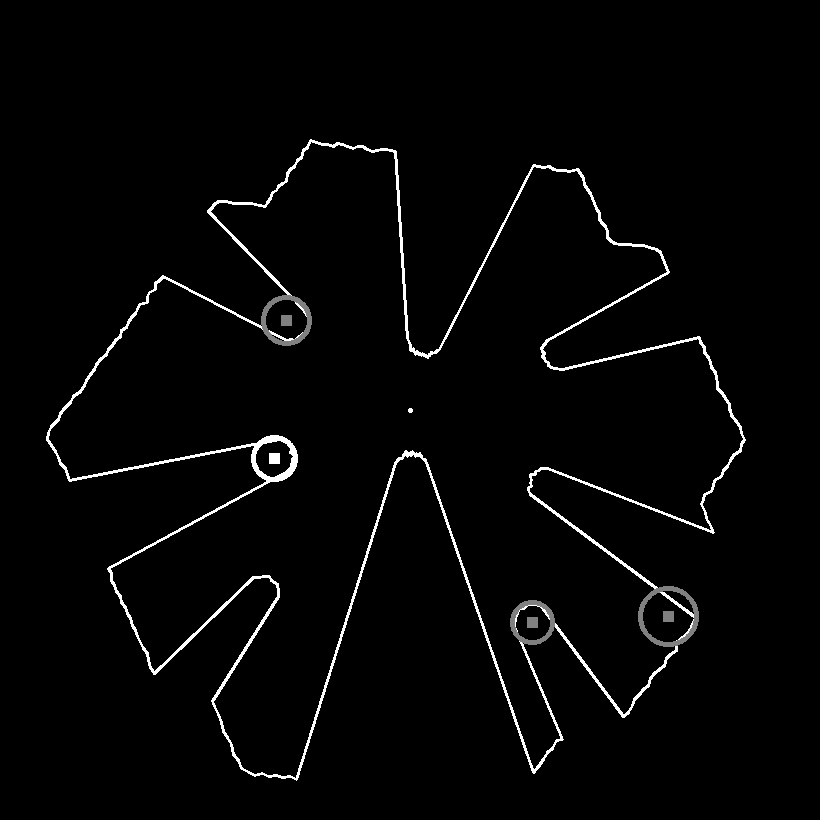
\includegraphics[width=7cm]{figs/circle_detection_sim}
    \caption{Detector de círculos en simulación.}
    \label{fig:circle_detection_sim}
  \end{minipage}
  \hfill
  \begin{minipage}{0.45\textwidth}
    \centering
    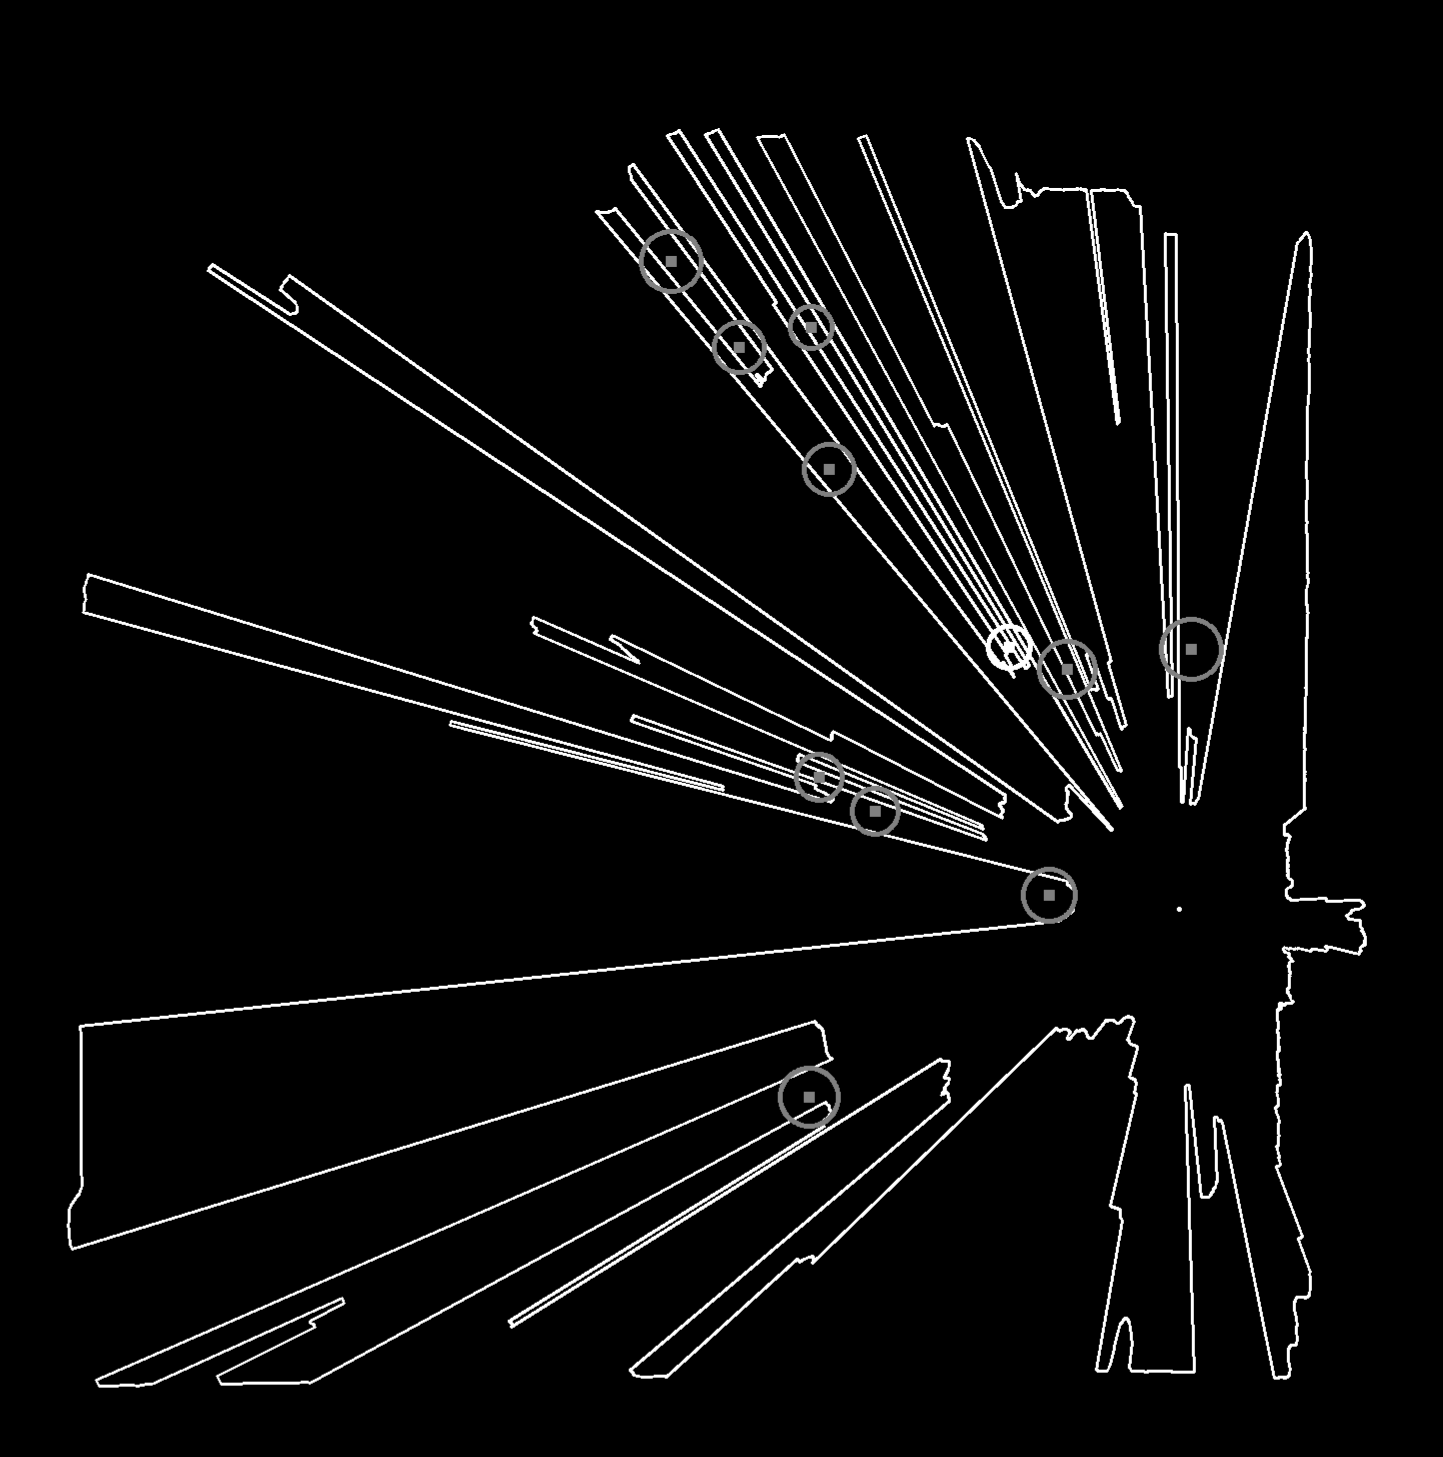
\includegraphics[width=7cm]{figs/circle_detection_lab}
    \caption{Detección de círculos en el laboratorio.}
    \label{fig:circle_detection_lab}
  \end{minipage}
\end{figure}\

Es por este motivo que se probó en un espacio más reducido, de aproximadamente
2x2m², como se puede ver en la Figura \ref{fig:lab_2x2_photo}, ya que cuanto más
grande sea el espacio, más grande deberá ser la resolución de la imagen
generada, lo que ralentizará la detección.
Con esta nueva configuración se obtuvo un mejor resultado, como se puede ver en
el Cuadro \ref{tab:circle_results_2x2}.

\begin{table}[h!]
\begin{center}
\begin{tabular}{|c|c|c|c|}
\hline
\textbf{Tamaño [px²]} & \textbf{Resolución [px/m]} & \textbf{Latencia [s]} & \textbf{Detección [\%]} \\
\hline
350x350 & 75  & 0.7 & 33  \\
450x450 & 100 & 0.8 & 100 \\
560x560 & 125 & 1.1 & 100 \\
880x880 & 200 & 1.3 & 93  \\
\hline
\end{tabular}
\caption{Resultados del nodo detector de círculos en un espacio de 2x2m²}
\label{tab:circle_results_2x2}
\end{center}
\end{table}

\begin{figure}[h!]
  \centering
  \begin{minipage}{0.45\textwidth}
    \centering
    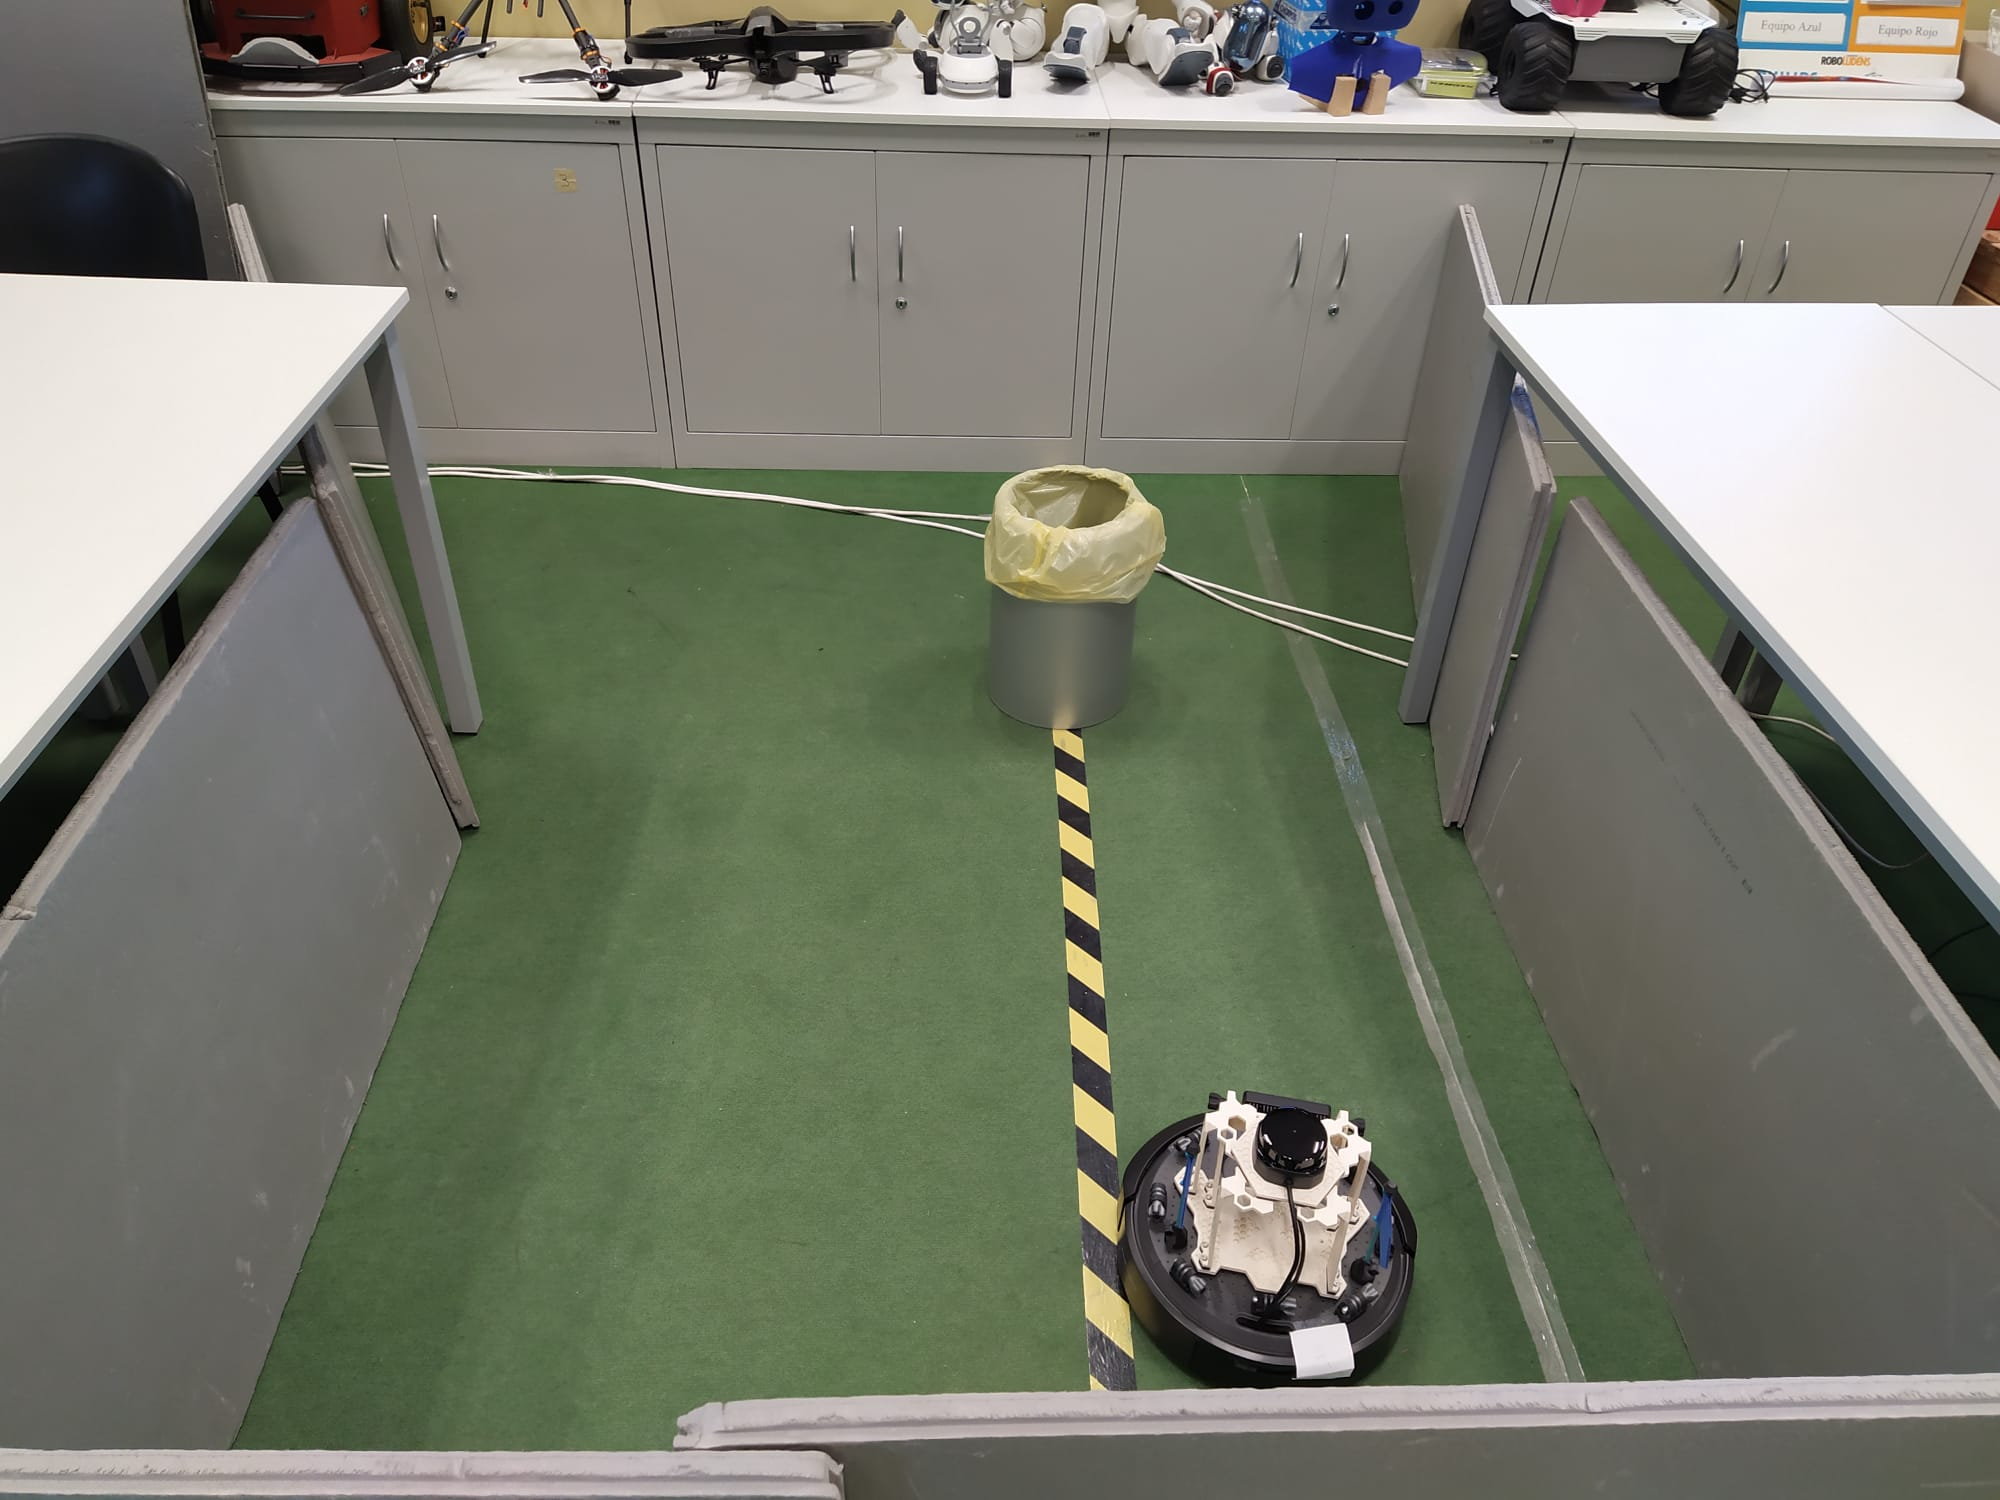
\includegraphics[width=7cm]{figs/lab_2x2_photo}
    \caption{Espacio de 2x2m² (aprox.)}
    \label{fig:lab_2x2_photo}
  \end{minipage}
  \hfill
  \begin{minipage}{0.45\textwidth}
    \centering
    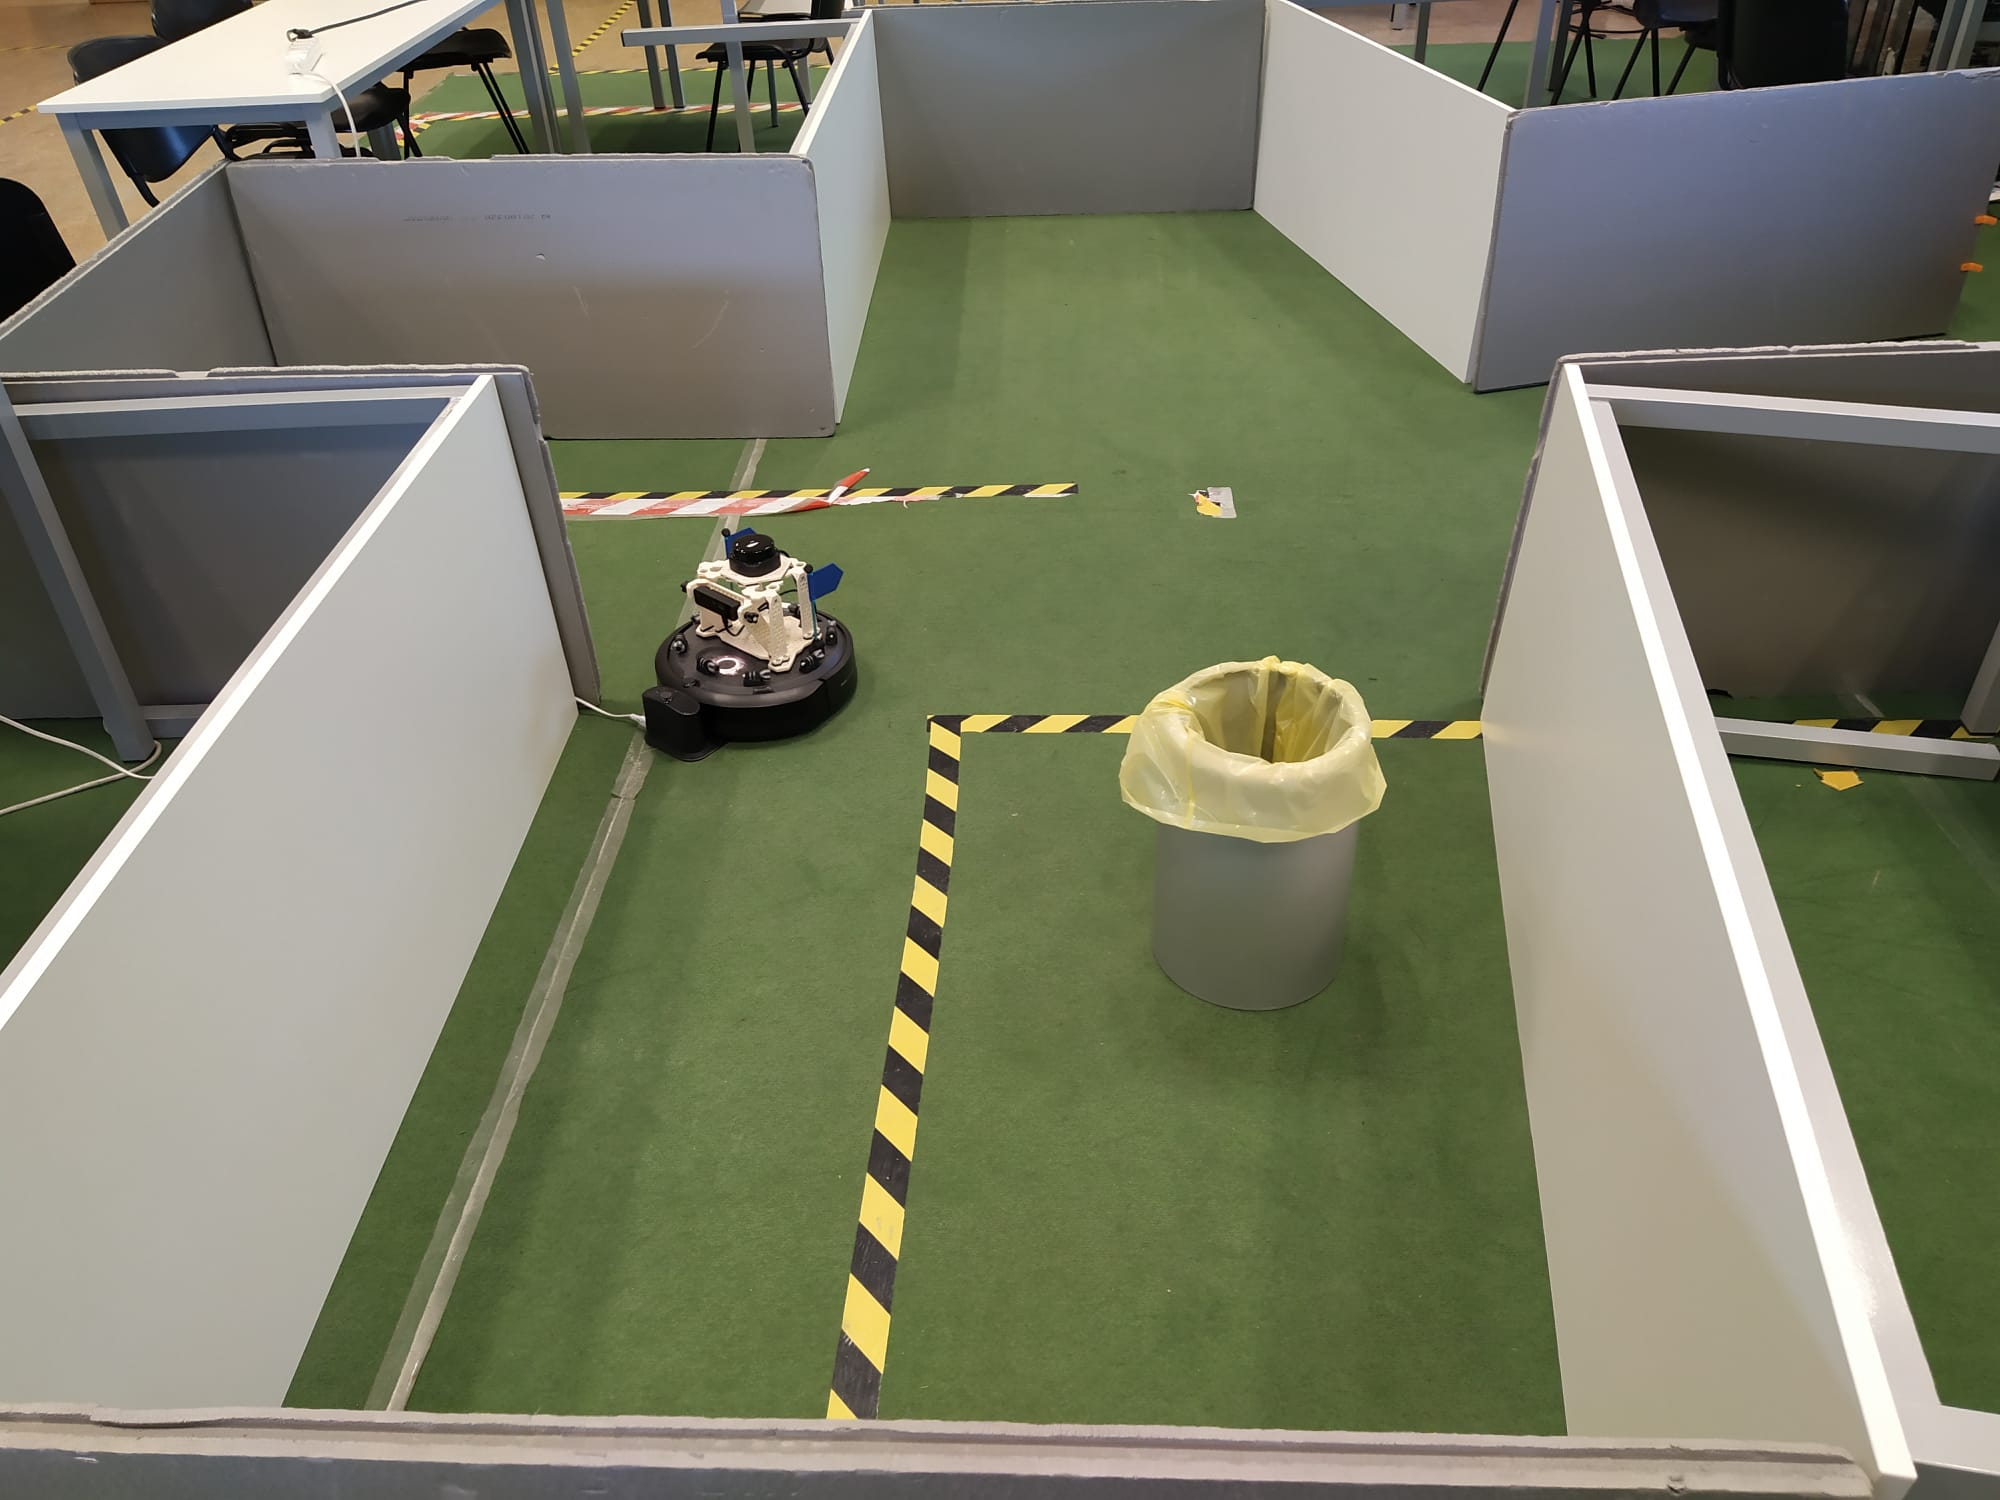
\includegraphics[width=7cm]{figs/lab_6x6_photo}
    \caption{Espacio de 6x6m² (aprox.)}
    \label{fig:lab_6x6_photo}
  \end{minipage}
\end{figure}\

Dadas las mejoras en la detección, se decidió ampliar el espacio a 6x6m²
aproximadamente, como puede verse  en la Figura \ref{fig:lab_6x6_photo}, para
poder realizar pruebas más robustas, en las que comparar el anterior algoritmo
con uno nuevo, que limitaba la distancia máxima detectada, creando siempre una
imagen igual o más pequeña, aunque limitando su rango de detección.
Estos resultados pueden verse en el Cuadro \ref{tab:circle_results_6x6}, en el
que se han probado ambos algoritmos con la misma resolución (100 px/m).
\\

\begin{table}[h!]
\begin{center}
\begin{tabular}{|c|c|c|c|c|}
\hline
\textbf{Tamaño [px²]} & \textbf{Res. [px/m]} & \textbf{Rango máx. [m]} & \textbf{Lat. [s]} & \textbf{Detección [\%]}  \\
\hline
888x888 & 100 & -   & 0.8 & 62  \\
672x672 & 75  & -   & 0.5 & 53  \\
\hline
425x425 & 100 & 2   & 0.2 & 35  \\
425x425 & 100 & 1.5 & 0.1 & 57  \\
\hline
\end{tabular}
\caption{Resultados del nodo detector de círculos en un espacio de 6x6m²}
\label{tab:circle_results_6x6}
\end{center}
\end{table}

Las detecciones obtenidas en ambos espacios, 2x2 y 6x6 m², pueden apreciarse en
las Figuras \ref{fig:lab_2x2} y \ref{fig:lab_6x6}, respectivamente.
\\

\begin{figure}[h!]
  \centering
  \begin{minipage}{0.45\textwidth}
    \centering
    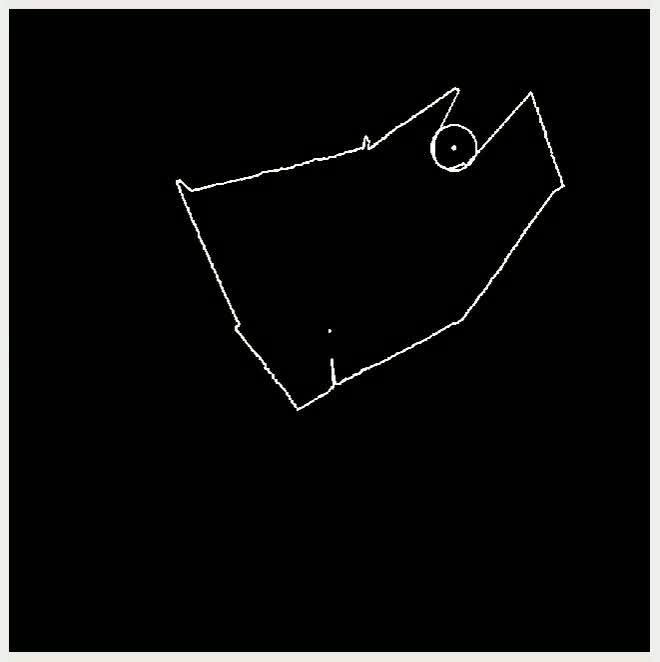
\includegraphics[width=7cm]{figs/lab_2x2}
    \caption{Detección en espacio de 2x2m² (aprox.)}
    \label{fig:lab_2x2}
  \end{minipage}
  \hfill
  \begin{minipage}{0.45\textwidth}
    \centering
    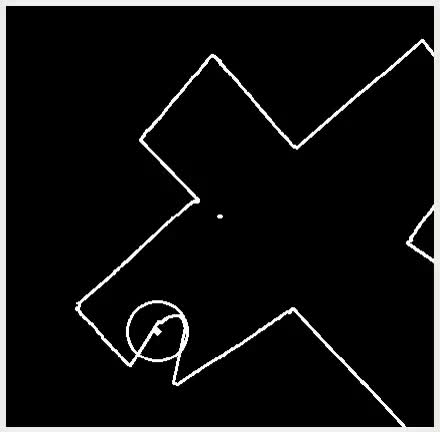
\includegraphics[width=7cm]{figs/lab_6x6_max2m}
    \caption{Detección en espacio de 6x6m² (aprox.) con rango máx. de 2m}
    \label{fig:lab_6x6}
  \end{minipage}
\end{figure}\

A pesar de haber obtenido mejores resultados en cuanto a latencia, se obtuvieron
peores resultados en cuanto a la propia detección del círculo.
Además, es en este momento cuando notamos que las imágenes generadas no están
siendo actualizadas correctamente: imprimiendo por pantalla las marcas de
tiempo de los mensajes recibidos del LIDAR notamos que se estaban recibiendo
únicamente los primeros mensajes del sensor en bucle, sin recibir nuevos.
\\

Haciendo pruebas con distintos robots, sensores LIDARs, e incluso corriendo el
detector sin Zenoh-Flow o ningún otro \textit{software}, llegamos a la
conclusión de que era problema de Zenoh-Flow, por lo que contactamos con la
empresa ZettaScale para comentar el problema, y nos respondieron que el
suscriptor de Zenoh, creado cuando se lanza el flujo de datos de Zenoh-Flow,
comienza a almacenar mensajes en este momento, llenando su \textit{buffer}, y
provocando que los nuevos mensajes se pierdan, y probablemente este no se vacía
lo suficientemente rápido como para considerar los mensajes como nuevos, dando
lugar a una gran latencia.
\\



